\documentclass{article}

\usepackage[a4paper, margin=1.5cm]{geometry}

\usepackage{graphicx}
%\usepackage{subcaption}
\usepackage{array}
\usepackage{tabularx}
\usepackage{booktabs}
\usepackage{multicol,caption}
\setlength{\columnsep}{1cm}

\newenvironment{Figure}
{\par\medskip\noindent\minipage{\linewidth}}
{\endminipage\par\medskip}

%opening
\title{Project Documentation for \\Mathematics of Neural Networks}
\author{Johann Kipping}

\begin{document}

\maketitle

\begin{multicols}{2}

\begin{abstract}
The aim of this project is to test the learned things in the first half of the lecture series on Neural Networks on the example of the Fashion-MNIST Dataset\\
\\
Things that could be done on Fashion-MNIST
\begin{itemize}
	\item Hyperparameter search
	\item Activation functions
	\item Initialization
	\item Optimizers
	\item Regularization (Overfitting?) + Generality
	\item FFT/im2col/Winograd
	\item Attribution
	\item Feature Visualization
	\item Adversarial Attacks
	\item Going deep?
\end{itemize}
\end{abstract}

\section*{0\quad Getting TF to run with a GPU with CUDA CC of 3.0}
As this is a documentation of work it will be mentioned that a significant amount of time needed for the setup of computations was put into getting tensorflow to compute on the available GPU (Geforce 660 Ti). The major obstacle was the fact that this particular GPU has a \textit{CUDA compute capability} of 3.0. The least tensorflow supports as of now is 3.5. This lead to the necessity of \textbf{downgrading to tensorflow version 1.12}. This might impede the ability for coverage of advanced topics.

\section{Idea collection and planning}
\label{ideas}
This chapter aims to collect ideas to most of the topics that were discussed in the lecture and continues to formulate a plan on how to tackle them in this project work.\\
\\
Loss functions used is categorical cross entropy. Why not Mean squared or something else\\
\\
\textbf{Hyperparameters:}\\
Idea: Try several choices of hyperparameters to get a feel for the effects. Do this in a grid-like fashion.\\
\\
\textbf{Activation functions / network structure}\\
Idea: Test small network structures (fast trainable) for effect of structural changes and different choices of activation functions using knowledge from the lecture and Exercise 4 from sheet 6 as starting point for network evaluation.\\
\\
\textbf{Initialization}\\
Idea: Verify the validity of the three approaches discussed in the lecture. (Zero/Random/Known data)\\
\\
\textbf{Optimizers}\\
Idea: Use Adam for all computations to reduce complexity of project as it incorporates other approaches.\\
\\
\textbf{Regularization (Overfitting?) + Generality}\\
Idea: Test for overfitting and generalization with own pictures (for fun). Maybe try regularization if poor performance is observed.\\
\\
\textbf{FFT/im2col/Winograd}\\
Idea: Let tensorflow decide on the usage of different approaches as insight was achieved in the exercises and modifications are not cheap.\\
\\
\textbf{Attribution/Feature Visualization}\\
Idea: Visualize a net (with more layers) feature maps by using Saliency maps and grad-Cam. Try out guided backpropagation if possible! Relu has to be used! Gradient ascent (google feature visualization)!\\
Neuron/Channel/Layer(DeepDream)
\\
\textbf{Adversarial Attack}\\
Idea: Use an adversarial attack to trick a net.\\
\\
\textbf{RNN}\\
Not the right datasets\\
\\
\textbf{ResNets}\\
Maybe? Lesioning!
\\
\\
Everything plot not shown in this documentation will be available in the github project.

\section{Getting to know Neural Networks}
This section will describe the first set of investigative experiments. Mainly regarding stuff of the first couple of lectures its main aim is to allow to get an understanding and feeling for the behavior of Neural Networks.

\subsection{Starting out}
As a starting point the network structure from Exercise 4 of sheet 6 was chosen to allow further investigation. As described in section \ref{ideas} Adam was be used as the optimizer throughout this section in order to reduce complexity.

\subsection{Initialization experiments}
The methods for initializations are to be tested in this section:
\begin{itemize}
	\item zero
	\item known data
	\item random
\end{itemize}
As mentioned before the net structure used for this will be structure from Exercise 4 of sheet 6.\\
The random initialization will be employed before the known data approach as the results from the random initialization will be used as the known data.
\subsubsection{Zero initialization}
As expected little to no improvement can be seen from training.

\subsubsection{Random initialization}
The baseline performance seen in the exercise. Uniform he initializer was used.

\subsubsection{Known data initialization}
This method allow the last two dense layers for classification to be further trained. This improved the networks performance for the training data, not for the test data
\begin{Figure}
	\label{fig:known_init}
	\centering
	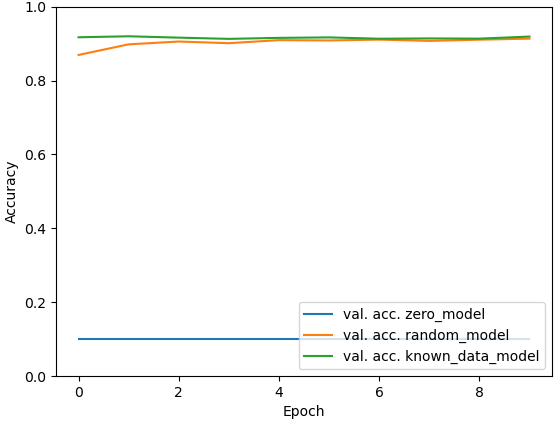
\includegraphics[width=\linewidth]{../img_1_1_init/acc_plot_init}
	\captionof{figure}{}
\end{Figure}

The resulting argument to be made is that form now on random initialization will be used due to lacking of known data. Zero initialization is not to be used.

\subsection{Hyperparameters for baseline network}
\label{hyperparams}
The hyperparameters for the fixed network structure of the baseline network with Adam as a fixed optimizer are batch size, epochs, learning rate, activation functions and initializers. The latter two have been or will be examined at another point in this documentation. In the following part a small grid-like search is employed.\\
\\
\begin{centering}
	\begin{tabular}{c c c c}
		%\toprule[2pt]
		 & 64 & 128 & 256 \\
		\toprule[2pt]
		.01 & 0.91  & 0.87 & 0.1 \\
		\midrule[0.2pt]
		.001 & 0.91  & 0.91 & 0.9 \\
		\midrule[0.2pt]
		.0001 & 0.89  & 0.89 & 0.88 \\
		\bottomrule[2pt]\\
		\multicolumn{4}{c}{Epochs: 5}
	\end{tabular}
	\hfill
	\begin{tabular}{c c c c}
		%\toprule[2pt]
		& 64 & 128 & 256 \\
		\toprule[2pt]
		.01 & 0.1  & 0.87 & 0.1 \\
		\midrule[0.2pt]
		.001 & 0.92  & 0.91 & 0.91 \\
		\midrule[0.2pt]
		.0001 & 0.91  & 0.9 & 0.9 \\
		\bottomrule[2pt]\\
		\multicolumn{4}{c}{Epochs: 20}
	\end{tabular}
\end{centering}

Different training times\\
Curve appearance/saturation

\subsection{Network structure}
The goal with changing network structure is to achieve better approximation of the wanted function. In this section three different approaches are chosen to try to increase performance. \\
\begin{enumerate}
	\item Increasing the number of neurons/filters motivated by the universal approximation theorem.
	\item Going deeper: allow for more steps of abstraction by increasing the numer of layers.
	\item Combining previous approaches and testing performance for different activation functions.
\end{enumerate}
The starting point for the hyperparameters will be those taken from section \ref{hyperparams}.

\subsubsection{UAT: Going wider}
In trying to reach a higher test accuracy the approach to use more neurons, motivated by the universal approximation theorem was taken.\\
The structure use in the previous sections was modified to use 4 times the amount of filters for the convolutional layers.\\
\\
Results did not show a visible improvement in testing accuracy neither for increasing the numer of filter in the convolutional layers nor the dense classification layers. This could indicate overfitting which will be investigated in section \ref{regularization}. A clear bottleneck for computation here was the rather tiny 2 GiB of memory on the GPU.\\
\\
To investigate the effects of increasing the number of neurons anyway a network structure with a flattening and one dense hidden layer is chosen and tested for the effect of having more neurons. The results show minimal improvement even for 32 times more neurons.

\subsubsection{Going deeper}
\label{deeper}
Another trick up the network designers sleeve is making the network deeper. As soon as another network structure was tried out and no improvement was observed a harder dataset had to be consulted as it seemed as though the baseline net was near optimal for Fashion-MNIST in the sense of efficient implementation with the tools at hand in the last couple of sections.\\
\\
The next step was then to try the CIFAR-10 dataset with the baseline net and compare the performance to a deeper version of the net. This resulted in a better performance at last but the high difference in the training accuracy and validation accuracy is still observable. This will be tackled by the regularization attempts in the following section.

\subsubsection{Activation functions}
At this point it should be investigated why the baseline net contains the activations it does. To this end the following was modifications were made and analyzed for the effects in training and validation accuracy:\\
\\
Several activation functions were tested for the baseline net to \textbf{replace ReLU}:\\
\\
\textbf{Elu}: The exponential ReLU activation performed marginally worse than ReLU in all tests with the baseline net.\\
\\
\textbf{Sigmoid}: The sigmoid function showed very low training and validation accuracy although with a monotone increase until the last epoch. The difference of training and validation accuracy was smaller than the other activation functions. \\
\\
\textbf{Tanh}: The tangens hyperbolicus outperformed all other functions and will investigated further in later sections.

\begin{Figure}
	\label{fig:known_init}
	\centering
	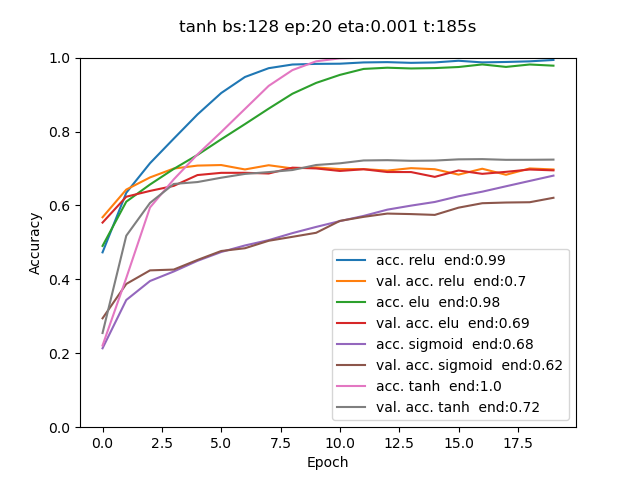
\includegraphics[width=\linewidth]{../img_1_4_activation/activation_comp}
	\captionof{figure}{}
\end{Figure}

\section{Regularization}
\label{regularization}
\subsection{Possible methods}
\begin{itemize}
	\item Depending on the Eigen/Singular Values vanishing/exploding gradients. As ReLU was used this is not regarded as possible.
	\item Bias very negative -> Dying neurons -> use leaky ReLU.
	\item Gradient clipping used for keeping out of saturation where gradient is almost zero -> usage of ReLU makes this probable to be unsuccessful
	\item Tikhonov ($L^{2}$) -> insert penalizing term into minimization to prevent weights getting to large. (Frobenius norm has to be used)
	\item Batch normalization -> normalize input to layers
	\item Dropout (Dropconnect) -> drop output of neurons with probability for each minibatch
\end{itemize}
As the previous chapter revealed the use of ReLU is acceptable for the baseline net with only tanh outperforming ReLU. To reduce the complexity in this section ReLU will thus be used. This renders the problem of vanishing/exploding gradients improbable such that gradient clipping and $L^{2}$ regularization will not be applied. The effects of the remaining methods are explored in the following sections.

\subsection{Dying neurons}
Using leaky ReLU to lower the possibility of neurons ''dying'' resulted in minor improvement as can be seen in figure \ref{fig:dying}
\begin{Figure}
	\label{fig:dying}
	\centering
	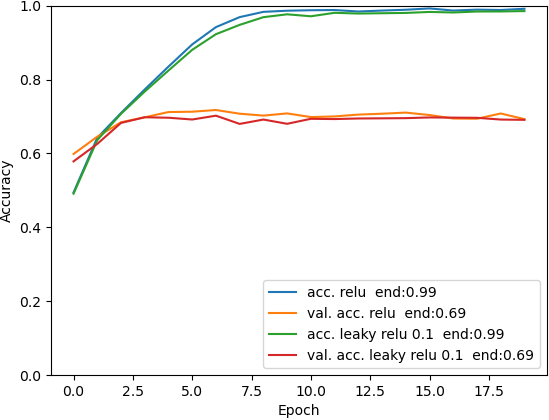
\includegraphics[width=\linewidth]{../img_1_5_regularization/dying}
	\captionof{figure}{}
\end{Figure}

\subsection{Batch normalization}
To make the input more readable for the net we normalize each element of the input to every layer to have mean $\mu=0$ and variance $\sigma=1$. To restrict less we learn parameters (linear transformation) $\beta and \gamma$ during backpropagation. Usage of ReLU\\
\\
For the baseline net the observed improvement was minimal, but for the deeper net from section \ref{deeper} there was a notable improvement especially in the time of convergence.

\begin{Figure}
	\label{fig:batchnorm}
	\centering
	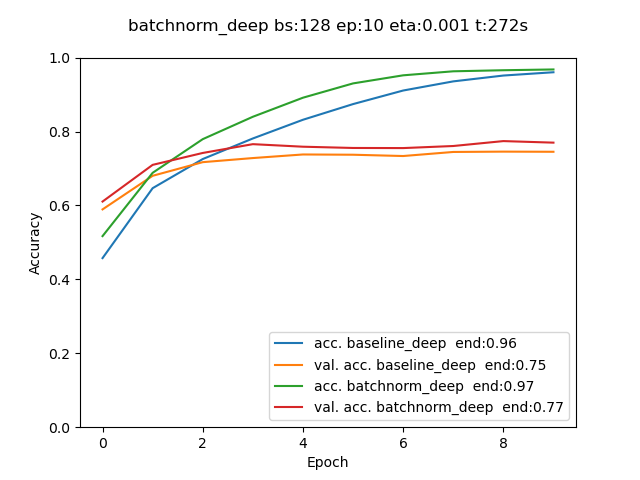
\includegraphics[width=\linewidth]{../img_1_5_regularization/batchnorm_deep}
	\captionof{figure}{}
\end{Figure}

\subsection{Dropout}
Localized features, more specialized filters

\begin{Figure}
	\label{fig:dropout}
	\centering
	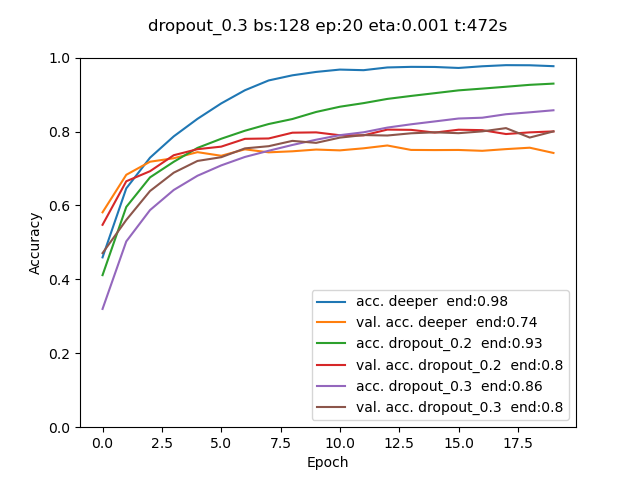
\includegraphics[width=\linewidth]{../img_1_5_regularization/dropout}
	\captionof{figure}{}
\end{Figure}

\section{Putting it all together}

Also testing with own picture

\section{Attribution}
Switching back to Fashion-MNIST\\


Check for generality and attribute in the same step by using an image from the test set and an image that was taken by me\\
\\
Using gradient tape -> saliency map\\
Global average pooling -> class activation map\\
Grad-CAM! am ehesten

\section{Adversarial attacks}

\section{Autoencoders}

\section{Generating new \textit{fashionable} clothing}

\end{multicols}
\end{document}
